\documentclass[osajnl,twocolumn,showpacs,superscriptaddress,10pt,floatfix]{revtex4-1} %% use 11pt for Applied Optics
\usepackage{amsmath,amssymb,graphicx,float}
\usepackage[utf8]{inputenc}
\graphicspath{ {images/} }

\begin{document}

\title{Thyroid Disease Data Set Analysis}

\author{Ulises Jeremias Cornejo Fandos}
\affiliation{Licenciatura en Informatica - 13566/7, Facultad de Informatica, UNLP}

\author{Gaston Gustavo Rios}
\affiliation{Licenciatura en Informatica - 13591/9, Facultad de Informatica, UNLP}


\begin{abstract}
Resumen
\end{abstract}

%\begin{abstract}This template is provided to demonstrate options
%for using REV\TeX{}4-1 in preparing manuscripts for submission to
%JOSA A, JOSA B, \textit{Optics Letters}, and \textit{Applied Optics}. REV\TeX{}4-1 support
%for OSA journals was added September 2012 as a BETA and updated in April 2013. Users should obtain the
%REV\TeX{}4-1 package (\url{https://authors.aps.org/revtex4/}) and the OSA REV\TeX{}4-1 style files  (on the Author page of any OSA journal site). Authors in need of a length estimate because of page charge concerns can use the OSA REV\TeX{}4-1 template. The template will not yield an exact estimate but should provide a good approximation of the length of the page proof. Figures, large tables, and complex display math may still affect the estimate. Note that the two-column format is acceptable %for submission and will meet the needs of OSA peer review and production.
%\end{abstract}

\ocis{}% REPLACE WITH CORRECT OCIS CODES FOR YOUR ARTICLE
                          % NOTE: \ocis{} IS ALIASED TO \pacs{} BUT MUST
                          % FORMAT THE TERMS CORRECTLY FOR EACH JOURNAL

\maketitle %% required

%\onecolumngrid
%\tableofcontents

%\clearpage

%\twocolumngrid

\section{Introducción}

\subsection{Thyroid Disease Data Set }

El data set cuenta con un conjunto de 6 bases de datos. En general, estos conjuntos son muy similares y presentan muchos atributos, \textit{aproximadamente 29 atributos cada conjunto de datos}, siendo la mayoría booleanos o reales. El dominio del problema es el análisis de enfermedades de tiroides y se utiliza para su estudio un conjunto de datos otorgado por Garavan Institute. Cada conjunto de datos cuenta con aproximadamente 2800 ejemplos y una \textit{gran cantidad de datos faltante}. \\

El conjunto de datos seleccionado permite la clasificación de pacientes entre aquellos que tienen hipotiroidismo y aquellos que no. En su versión presenta un total de 3163 ejemplares de los cuales se conocen 26 atributos. \\

\subsubsection{Información de los atributos}

\begin{itemize}
    \item \textit{age}: Este atributo corresponde a la edad del paciente. En un valor numérico continuo que toma valores de $R$.
    \item \textit{sex}: Este atributo corresponde al sexo del paciente. Toma valores del conjunto $\{M, F\}$ y presenta valores faltante.
    \item \textit{on\_thyroxine}:  \textit{Thyroxine} es la principal hormona generada por la glándula tiroides. Cuando se detecta mucha thyroxine y triyodotironina entonces reduce la producción de hormonas \textit{(TSH)}. Relacionado con goitre, este es una forma de reconocer demasiada thyroxine, la cual es causada por hipertiroidismo. Muy poca es causada por hypotiroidismo. Toma valores del conjunto $\{f, t\}$.
    \item \textit{query\_on\_thyroxine}: Este atributo indica si fue medido \textit{on\_thyroxine}. Toma valores del conjunto $\{f, t\}$.
    \item \textit{on\_antithyroid\_medication}: Antithyroid es un medicamento que actúa sobre las hormonas tiroides. Este atributo indica si el paciente toma dicha medicación. Toma valores del conjunto $\{f, t\}$.
    \item \textit{thyroid\_surgery}: Este atributo indica si el paciente ha tenido una cirugía de tiroides. Toma valores del conjunto $\{f, t\}$.
    \item \textit{query\_hyphotiroid}: Este atributo indica si le fue consultado al paciente si tenía hipotiroidismo. Toma valores del conjunto $\{f, t\}$.
    \item \textit{query\_hyperthyroid}: Este atributo indica si le fue consultado al paciente si tenía hipertiroidismo. Toma valores del conjunto $\{f, t\}$.
    \item \textit{pregnant}: Este atributo indica si el paciente esta transitando un embarazo. Toma valores del conjunto $\{f, t\}$.
    \item \textit{sick}: Este atributo indica si el paciente estaba enfermo al tomar los datos. Toma valores del conjunto $\{f, t\}$.
    \item \textit{tumor}: Este atributo indica si el paciente tenía un tumor al tomar los datos. Toma valores del conjunto $\{f, t\}$.
    \item \textit{lithium}: Toma valores del conjunto $\{f, t\}$.
    \item \textit{goitre}: Toma valores del conjunto $\{f, t\}$.
    \item \textit{TSH\_measured}: Este atributo indica si se mide el \textit{TSH} del paciente. Toma valores del conjunto $\{f, t\}$.
    \item \textit{TSH}: Toma valores de $R$.
    \item \textit{T3\_measured}: Este atributo indica si se mide el \textit{T3} del paciente. Toma valores del conjunto $\{f, t\}$.
    \item \textit{T3}: Toma valores de $R$.
    \item \textit{TT4\_measured}: Este atributo indica si se mide el \textit{TT4} del paciente. Toma valores del conjunto $\{f, t\}$.
    \item \textit{TT4}: Toma valores de $R$.
    \item \textit{T4U\_measured}: Este atributo indica si se mide el \textit{T4U} del paciente. Toma valores del conjunto $\{f, t\}$.
    \item \textit{T4U}: Toma valores de $R$.
    \item \textit{FTI\_measured}: Este atributo indica si se mide el \textit{FTI} del paciente. Toma valores del conjunto $\{f, t\}$.
    \item \textit{FTI}: Toma valores de $R$.
    \item \textit{TBG\_measured}: Este atributo indica si se mide el \textit{TBG} del paciente. Toma valores del conjunto $\{f, t\}$.
    \item \textit{TBG}: Toma valores de $R$.
\end{itemize}

\subsection{Recolección del conjunto de datos}

El conjunto de datos seleccionado se obtiene del repositorio \textit{thyroid disease} del conjunto de data sets para machine learning de \textit{archive.ics.uci.edu}. Como se menciona anteriormente, en el mismo existe una gran cantidad de bases de datos y del mismo se opta por utilizar un conjunto de datos agregado más recientemente. \\

En la descripción del mismo se duda de la integridad de los datos pero se comenta que de igual forma el otorgante es Garavan Institute al igual que el resto de los data sets. A su vez, no dice en ningun momento como es que estos datos son recolectados por lo que al momento de analizar estos datos, solo conocemos las fuentes utilizadas y la entidad otorgante. \\

\section{Pre-procesamiento de datos}
\subsection{Conjunto a analizar}

Como se explica en la sección anterior, existen atributos en los cuales se muestra si fue medido un atributo o no. Dado que los valores de estos coinciden con los datos faltantes se opta por la eliminación de dichos atributos. Al mismo tiempo, la cantidad de datos faltantes para la columna correspondiente al atributo TBG es \textbf{PORCENTAJE y SOLUCION}. Teniendo en cuenta esto, se opta por la eliminación de dicha columna dado que se considera que la misma podría llegar a interferir en el proceso del análisis de los datos, quedando finalmente un total de 19 atributos y 3163 ejemplos. \\

Luego se resuelven los datos faltantes de cada atributo utilizando la media de los mismos para los datos continuos y el valor de mayor frecuencia para los valores nominales. Se mapea el valor correspondiente al atributo sexo para que tome valores del conjunto $\{Male, Female\}$, y aquellos atributos booleanos para que los valores pasen de $f$ a $False$ y de $t$ a $True$. \\

\section{Marco Teórico}

En esta sección se introduce brevemente conceptos básicos necesarios para abordar los contenidos de las siguientes secciones del informe con mayores referencias y capacidad de entendimiento. \\

\subsection{Árbol de decisión}

Modelo descriptivo que, por su forma jerarquica, permite visualizar la organización de los atributos. Se produce a partir de la identificación sucesiva de atributos relevantes. El atributo correspondiente a la clase es cualitativo.

\subsection{Árbol de clasificación}

Es un Arbol de decisión cuyas hojas se refieren al mismo atributo y es discreto.

\subsection{Reglas de clasificación}

Modelo supervisado que apartir de la información busca obtener reglas de la forma: $ A \rightarrow B $. \\

Comparado con el modelo explicado en la subsección anterior, las reglas de clasificación son más compactas que los arboles en donde cada regla puede representar un concepto distinto permitiendo así agregar o quitar reglas dinamicamente.

\subsection{Clustering}

Un algoritmo de agrupamiento (en inglés, clustering) es un procedimiento de agrupación de una serie de vectores de acuerdo con un criterio. Esos criterios son por lo general distancia o similitud. La cercanía se define en términos de una determinada función de distancia, como la euclídea, aunque existen otras más robustas o que permiten extenderla a variables discretas. La medida más utilizada para medir la similitud entre los casos es la matriz de correlación entre los nxn casos. Sin embargo, también existen muchos algoritmos que se basan en la maximización de una propiedad estadística llamada verosimilitud. \\

En el contexto de la Mineria de Datos se lo considera una técnica de aprendizaje no supervisado puesto que busca encontrar relaciones entre variables descriptivas pero no la que guardan con respecto a una variable objetivo. \\

\subsubsection{K-Means}

\textbf{K-means} es un método de agrupamiento, que tiene como objetivo la partición de un conjunto de n observaciones en k grupos en el que cada observación pertenece al grupo cuyo valor medio es más cercano. \\

En la figura \ref{figure:clustering_example} se muestra un ejemplo de aplicación del algoritmo k-means para realizar un agrupamiento de los datos.

\begin{figure}[H]
    \centering
    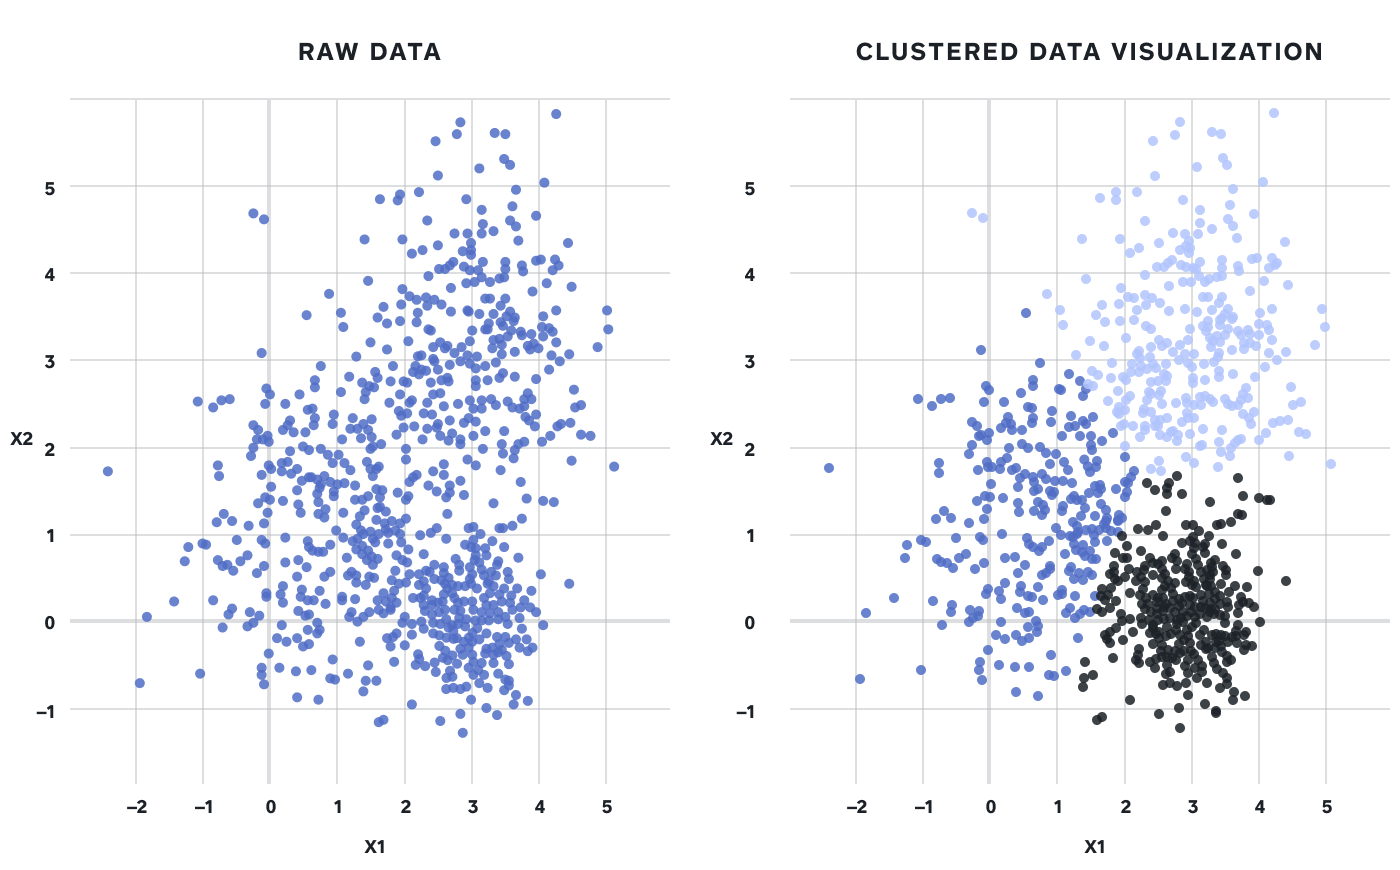
\includegraphics[width=0.4\textwidth]{theory/clustering}
    \caption{Ejemplo de aplicación del algoritmo k-means para realizar un agrupamiento de los datos.}
    \label{figure:clustering_example}
\end{figure}

\subsection{Redes Neuronales}

Las \textbf{redes neuronales} son un modelo computacional basado en un gran conjunto de unidades neuronales simples, \textbf{neuronas artificiales}, de forma aproximadamente análoga al comportamiento observado en los axones de las neuronas en los cerebros biológicos. \\

Cada unidad neuronal está conectada con muchas otras y los enlaces entre ellas pueden incrementar o inhibir el estado de activación de las neuronas adyacentes. Cada unidad neuronal, de forma individual, opera empleando funciones de suma. Puede existir una función limitadora o umbral en cada conexión y en la propia unidad, de tal modo que la señal debe sobrepasar un límite antes de propagarse a otra neurona. \\

Estos sistemas aprenden y se forman a sí mismos, en lugar de ser programados de forma explícita, y sobresalen en áreas donde la detección de soluciones o características es difícil de expresar con la programación convencional.

\subsubsection{Perceptron}

En el campo de las Redes Neuronales, el \textbf{perceptrón}, se refiere a la neurona artificial o unidad básica de inferencia en forma de discriminador lineal, a partir del cual se desarrolla un algoritmo capaz de generar un criterio para seleccionar un sub-grupo a partir de un grupo de componentes más grande. \\

En la figura \ref{figure:perceptron_example} se muestra la arquitectura que determina el comportamiento de un perceptron.

\begin{figure}[H]
    \centering
    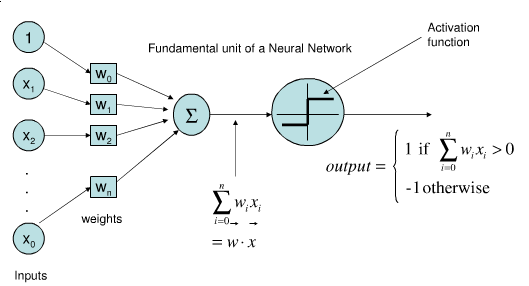
\includegraphics[width=0.4\textwidth]{theory/perceptron}
    \caption{Arquitectura de un perceptron.}
    \label{figure:perceptron_example}
\end{figure}

La limitación de este algoritmo es que si dibujamos en un gráfico estos elementos, se deben poder separar con un hiperplano únicamente los elementos "deseados" discriminándolos (ó \textit{separándolos}) de los \textit{"no deseados"} como se muestra en la figura \ref{figure:linear_example}.

\begin{figure}[H]
    \centering
    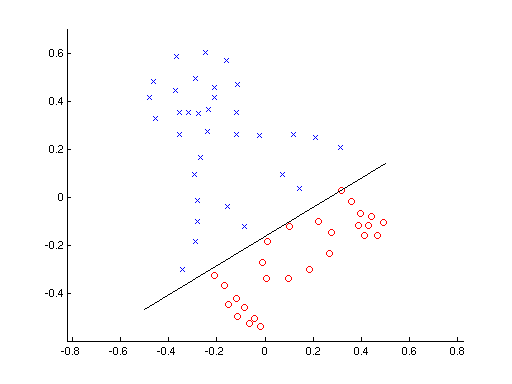
\includegraphics[width=0.4\textwidth]{theory/linear}
    \caption{Ejemplo de función linear discriminante.}
    \label{figure:linear_example}
\end{figure}

El perceptrón puede utilizarse con otros tipos de perceptrones o de neurona artificial, para formar una red neuronal artificial más compleja.

\subsubsection{Multiperceptrón}

El \textbf{perceptrón multicapa}, \textit{multi-perceptrón}, es una red neuronal artificial formada por múltiples capas, de tal manera que tiene capacidad para resolver problemas que no son linealmente separables que, como se explica en la subsección anterior, es la principal limitación del \textit{perceptrón}. El perceptrón multicapa puede estar totalmente o localmente conectado. En el primer caso cada salida de una neurona de la capa \textit{"i"} es entrada de todas las neuronas de la capa \textit{"i+1"}, mientras que en el segundo cada neurona de la capa \textit{"i"} es entrada de una serie de neuronas (región) de la capa \textit{"i+1"}. \\

Se muestra en la figura (\ref{figure:multiperceptron_example}) un ejemplo de la arquitectura de un perceptron multicapa.

\begin{figure}[H]
    \centering
    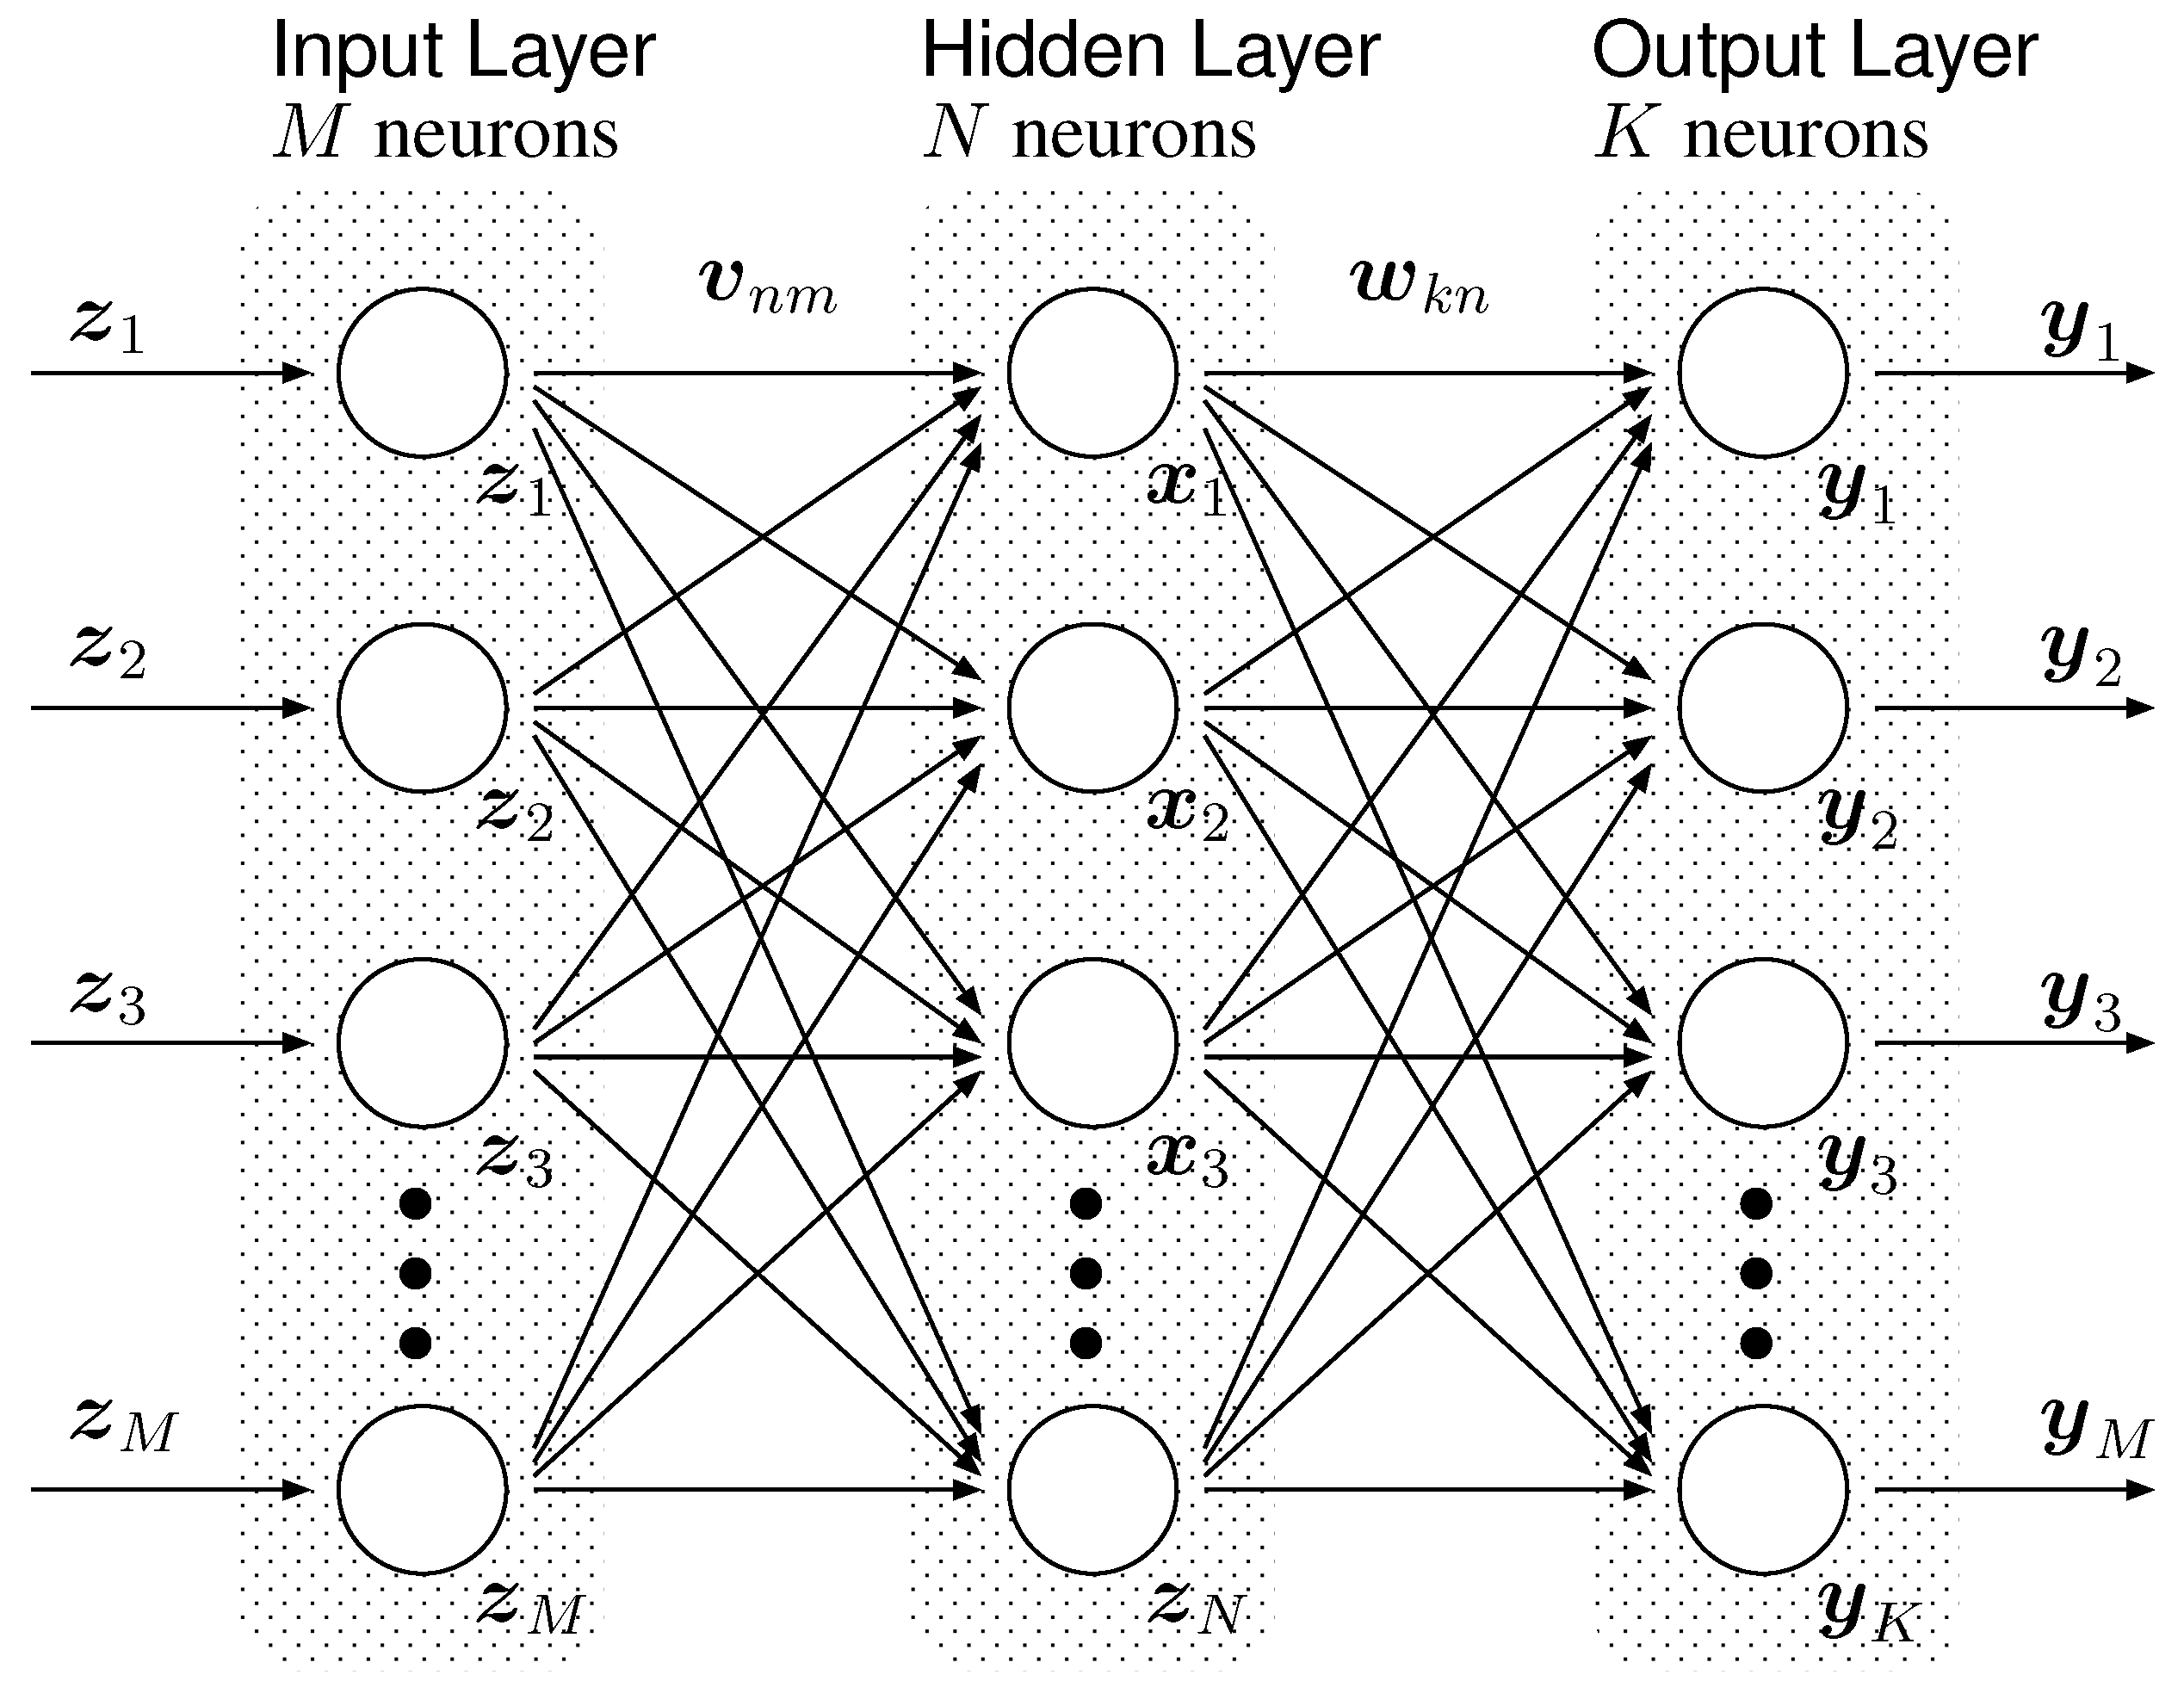
\includegraphics[width=0.4\textwidth]{theory/multiperceptron}
    \caption{Ejemplo básico de un multiperceptron.}
    \label{figure:multiperceptron_example}
\end{figure}

\section{Análisis de datos}

Para el análisis de los datos se evalúan distintas gráficas de lo mismos, como histogramas de los datos nominales y gráficas de dispersión para aquellos datos de tipo numérico, además de ciertas métricas que permiten conocer la correlación entre cada uno de ellos. De este modo se permite observar relaciones entre los distintos atributos del conjunto de datos así como también la relación entre estos mismos y la etiqueta, o \textit{label}.

\begin{flushright}
\textit{\footnotesize Se dispone de las gráficas correspondientes a los atributos en la sección \ref{apendix:images:attr} del apéndice.}
\end{flushright}

Posteriormente, se calcula el índice de correlación lineal entre los atributos, para comenzar así con el análisis de las relaciones entre cada uno de ellos. El cálculo de los mismos se ve reflejado en la siguiente tabla (\ref{table:correlation_matrix}). \\

\begin{table}[h!]
    \centering
    \begin{tabular}{ccccccc}

        Atributos & age & TSH & T3 & TT4 & TU4 & FTI \\
        \hline
        age & 1 & -0.007 & -0.269 & -0.091 & -0.194 & 0.015 \\

        TSH & -0.007 & 1 & -0.172 & -0.310 & 0.069 & -0.244 \\
        
        T3 & -0.269 & -0.172 & 1 & 0.545 & 0.388 & 0.294 \\
        
        TT4 & -0.091 & -0.310 & 0.545 & 1 & 0.323 & 0.685 \\
        
        T4U & -0.194 & 0.069 & 0.388 & 0.323 & 1 & -0.284 \\
        
        FTI & 0.015 & -0.244 & 0.294 & 0.685 & -0.283 & 1 \\
        \hline
    \end{tabular}
    \caption{Matriz de correlación lineal}
    \label{table:correlation_matrix}
\end{table}

Como se observa en la tabla 1, las tuplas (FTI, TT4) y (T3, TT4) presentan una correlación lineal leve, con un índice de correlación de 0.685 y 0.545 respectivamente. \\

\section{Método Experimental}

En esta sección se detalla todo lo referido al estudio y la creación de los distintos modelos de sistemas inteligentes utilizados para el estudio del conjunto de datos elegido. \\

\subsection{Árbol de decisión}

Para la creación del modelo de Árbol de decisión, se evalúan las distintas posibilidades permitiendo así la construcción de un modelo con un mayor nivel de cobertura sobre el conjunto de datos empleado para entrenamiento y prueba. \\

\textbf{EXPLICAR ELECCIÓN DEL MODELO} \\

Por lo tanto, como se menciona anteriormente, dado que el conjunto de datos presenta atributos numéricos de tipo continuo, no es completamente viable discretizar los mismos en intervalos si es que existe alguna forma de construir un modelo de Árbol de decisión evitando esto. \\

Se opta finalmente la utilización del algoritmo C4.5 para generar el Árbol de Decisión. Se genera el árbol utilizando el operador W-J48 de rapidminer con la configuración defecto de la mayoría de los flags exceptuando el flag C, \textit{confianza}. Luego de probar distintas configuraciones para el mismo, se observa que dado un conjunto de entrenamiento del 70\% del total de los datos, con un 30\% de los datos destinado al testing del modelo, el porcentaje de acierto del modelo es 99.59\% cuando $C \geq 0.5$, por lo que se configura el flag con $C$ con el valor $0.5$. \\

En la figura (\ref{figure:w_j48}) se puede observar el modelo obtenido utilizando el algoritmo C4.5.

\begin{figure}[H]
    \centering
    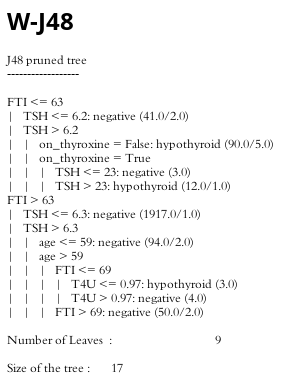
\includegraphics[width=0.35\textwidth]{models/w_j48}
    \caption{Modelo de Árbol generado utilizando el algoritmo C4.5, con una performance de 99.16\%.}
    \label{figure:w_j48}
\end{figure}

En la figura (\ref{figure:w_j48_performance}) de la sección \ref{apendix:models:performance} se puede observar la performance del modelo obtenido aplicando el mismo sobre un conjunto de testing. \\

\subsection{Reglas de Clasificación}

Para definir el algoritmo a utilizar para la creación de reglas se evalúa cada uno de ellos comparando los modelos generados para determinar así cual es más conveniente. Entre los algoritmos evaluados están OneR y PRISM. \\

\subsubsection{OneR}

Para la construcción de este modelo se trabaja con un conjunto normalizado de los datos utilizando normalización Z sobre los datos de tipo numérico. El antecedente de la regla generada por este algoritmo se define a partir del atributo $FTI$ como se puede observar en la figura (\ref{figure:w_oneR}). \\

\begin{figure}[H]
    \centering
    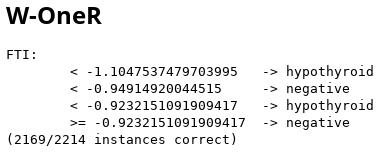
\includegraphics[width=0.4\textwidth]{models/w_oneR}
    \caption{Modelo generado por el algoritmo OneR.}
    \label{figure:w_oneR}
\end{figure}

En la figura (\ref{figure:w_oneR_performance}) de la seccion \ref{apendix:models:performance} se puede observar la performance del modelo obtenido aplicando el mismo sobre un conjunto de testing. \\

\subsubsection{PRISM}

Para la construcción del modelo de reglas utilizando el algoritmo PRISM se discretiza por frecuencia los datos numéricos probando le performance del modelo para distintos intervalos. Finalmente se opta por discretizar en 7 intervalos obteniendo los resultados que se muestran en la figura (\ref{figure:prism_performance}) de la sección \ref{apendix:models:performance}. \\

\textbf{CONTAR CANTIDAD DE REGLAS OBTENIDAS}

\section{Clustering}

\subsection{K-Means}

Para la construcción de este modelo se utiliza el algoritmo K-means evaluando las distancias con distancia euclidea. Se normalizan los datos utilizando normalización Z y se evalúa el modelo resultante utilizando el índice de Davies Bouldin notando que se obtiene mejores resultandos cuando el número de clusters $k$ es igual a 2, obteniendo finalmente un índice de Davies Bouldin igual a 0.601. \\

Como resultado se obtienen dos agrupamientos, \textit{cluster\_0} y \textit{cluster\_1}. En los mismos se ve que si el paciente pertenece al cluster\_0 no tiene hypotiroides. Al mismo tiempo, las instancias pertenecientes al cluster\_0 tienen TSH mas bajo, T3 mas alto, y TT4 y FTI bastante más alto que la media. Hay muy pocos que son de cluster\_0 y se pueden ver los datos del agrupamiento en la tabla (\ref{table:k_means}).


\begin{table}[h!]
    \centering
    \begin{tabular}{ccccccc}
        hypothyroid & cluster & cantidad \\
        \hline
        hypothyroid & cluster\_1 & 151.0 \\
        negative & cluster\_0 & 39.0 \\
        negative  & cluster\_1 & 2973.0 \\
        \hline
    \end{tabular}
    \caption{Resultados del clustering generado con k\_means}
    \label{table:k_means}
\end{table}

Los datos referidos al agrupamiento se pueden ver  en la sección \ref{apendix:models:performance} del apéndice. \\

\section{Redes Neuronales}

Se evalúan distintos modelos de redes neuronales con distintos conjuntos de prueba para evaluar así la performance de los mismos y comparar los modelos resultantes.

\subsection{Perceptrón}

Dado que el atributo etiqueta del data set es un es un conjunto de valores categóricos de cardinalidad igual a 2, se evalúa la utilización de un perceptrón como posible arquitectura de redes neuronales. \\

\textbf{Pesos y bias}

Como se menciona en el marco teórico, la función discriminante que define al perceptron se define en función de un Intercept y distintos pesos o coeficientes asociados a cada uno de los valores de los atributos del data set. A continuación se enlistan los valores obtenidos luego de entrenar el perceptron. \\

\textit{Intercept} = 1.3490659272630658 \\

En la tabla (\ref{table:perceptron_attr_weight}) se muestran los pesos asociados a cada atributo. \\

\begin{table}[ht]
    \begin{tabular}{l|l}
        Atributo & Peso \\
        \hline
        sex = Male & -0.006 \\
        sex = Female & 0.006 \\
        on\_thyroxine = False & -0.002 \\
        on\_thyroxine = True & 0.002 \\
        query\_on\_thyroxine = False & -0.203 \\
        query\_on\_thyroxine = True & 0.203 \\
        on\_antithyroid\_medication = False & -0.018 \\
        on\_antithyroid\_medication = True & 0.018 \\
        thyroid\_surgery = False & 0.009 \\
        thyroid\_surgery = True & -0.009 \\
        query\_hypothyroid = False & -0.046 \\
        query\_hypothyroid = True & 0.046 \\
        query\_hyperthyroid = False & -0.002 \\
        query\_hyperthyroid = True & 0.002 \\
        pregnant = False & -0.052 \\
        pregnant = True & 0.052 \\
        sick = False & -0.019 \\
        sick = True & 0.019 \\
        tumor = False & -0.295 \\
        tumor = True & 0.295 \\
        lithium = False & -1.955 \\
        lithium = True & 1.955 \\
        goitre = False & 0.001 \\
        goitre = True & -0.001 \\
        age & -0.016 \\
        TSH & 0.007 \\
        T3 & -0.025 \\
        TT4 & 0.232 \\
        T4U & -0.102 \\
        FTI & 0.438 \\
    \end{tabular}
    \caption{Tabla de pesos para cada atributo utilizando un perceptrón.}
    \label{table:perceptron_attr_weight}
\end{table}

En las figuras (\ref{figure:perceptron_performance}) y (\ref{figure:perceptron_train_test_performance}) de la seccion \ref{apendix:models:performance} se puede observar la performance del modelo obtenido aplicando el mismo sobre un conjunto de testing. \\

\subsection{Multiperceptron}

Se entrena un multiperceptron utilizando el operador NeuralNet de RapidMiner con 500 ciclos de entrenamiento, 0.03 de tasa de aprendizaje y momentum igual a 0.2, obteniendo una performance mayor a la obtenida con el modelo anterior. \\

En las figuras (\ref{figure:multiperceptron_performance}) y (\ref{figure:multiperceptron_train_test_performance}) de la seccion \ref{apendix:models:performance} se puede observar la performance del modelo de redes neuronales obtenido aplicando el mismo sobre un conjunto de testing. \\

\section{Análisis de Resultados}

\textbf{ANALISIS DE RESULTADOS}

\section{Discusión y Conclusiones}

\textbf{DISCUSION Y CONCLUSIONES}

\begin{thebibliography}{99}
%% Do not include separate BibTeX files; if BibTeX is used,
%% paste the output (contents of .bbl file) here.

\bibitem{revtex-au} \url{https://authors.aps.org/revtex4/}.
\bibitem{osastyle} \url{http://www.opticsinfobase.org/submit/style/jrnls_style.cfm}.

\end{thebibliography}

\clearpage

\onecolumngrid

\section{Apéndice}

\subsection{Imágenes} \label{apendix:images}

\subsubsection{Gráficos de los atributos} \label{apendix:images:attr}

\twocolumngrid

\begin{figure}[H]
    \centering
    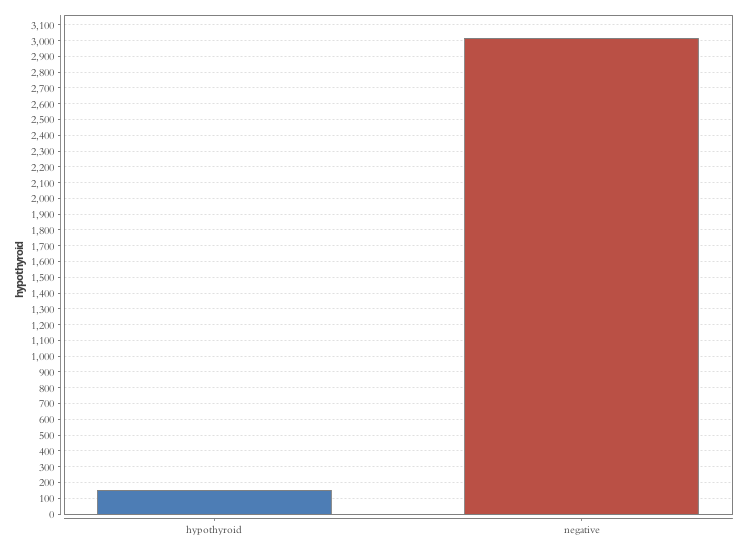
\includegraphics[width=0.45\textwidth]{analysis/bars_hypothyroid}
    \caption{Gráfico de barras del atributo etiqueta.}
    \label{figure:bars_hypothyroid}
\end{figure}

\begin{figure}[H]
    \centering
    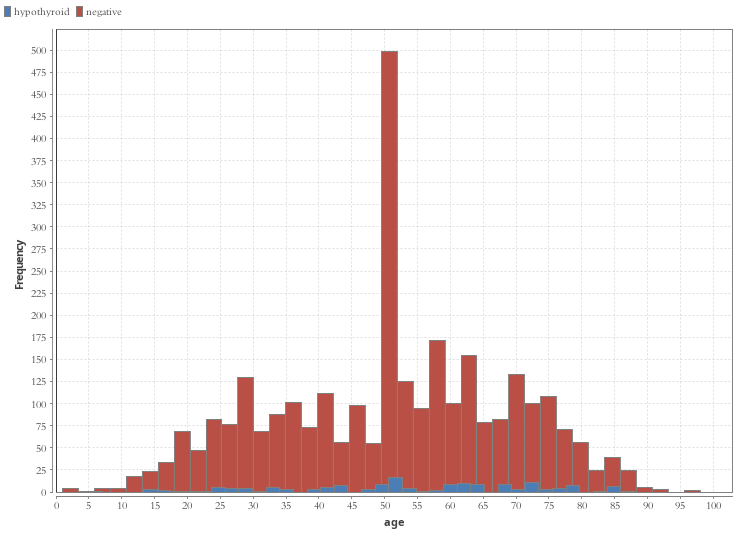
\includegraphics[width=0.45\textwidth]{analysis/histogram_age}
    \caption{Histograma del atributo \textit{age}.}
    \label{figure:histogram_age}
\end{figure}

\begin{figure}[H]
    \centering
    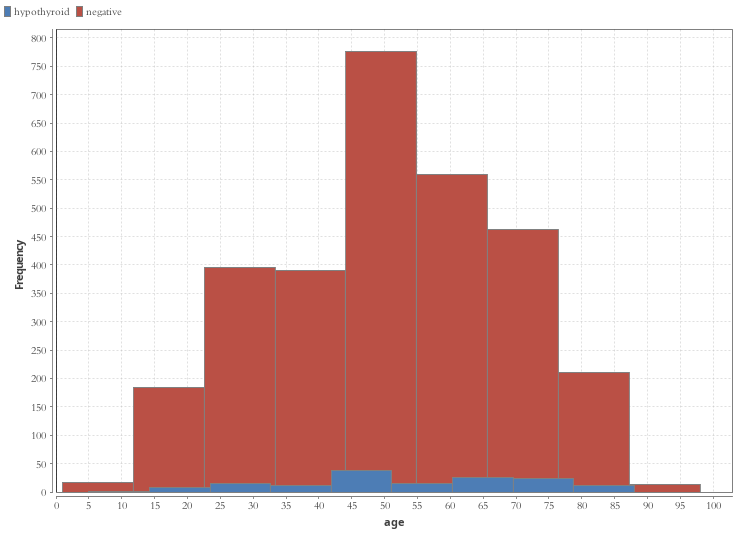
\includegraphics[width=0.45\textwidth]{analysis/histogram_age2}
    \caption{Histograma del atributo \textit{age}.}
    \label{figure:histogram_age2}
\end{figure}

\begin{figure}[H]
    \centering
    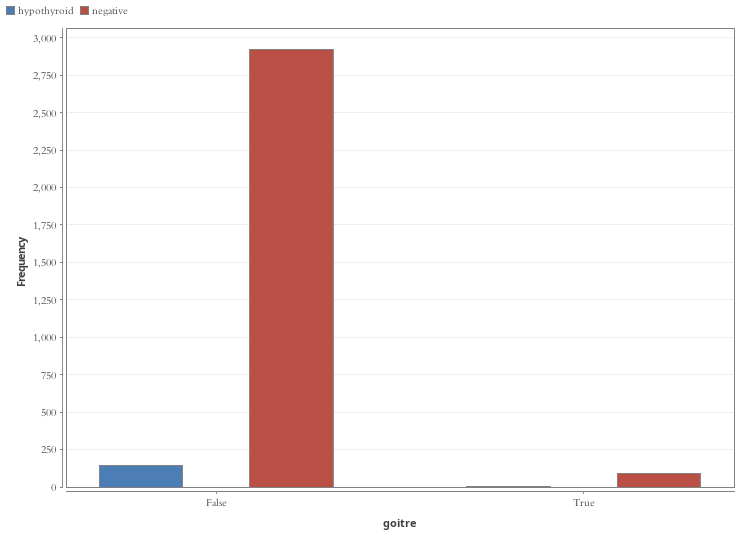
\includegraphics[width=0.45\textwidth]{analysis/histogram_goitre}
    \caption{Histograma del atributo \textit{goitre}.}
    \label{figure:histogram_goitre}
\end{figure}

\begin{figure}[H]
    \centering
    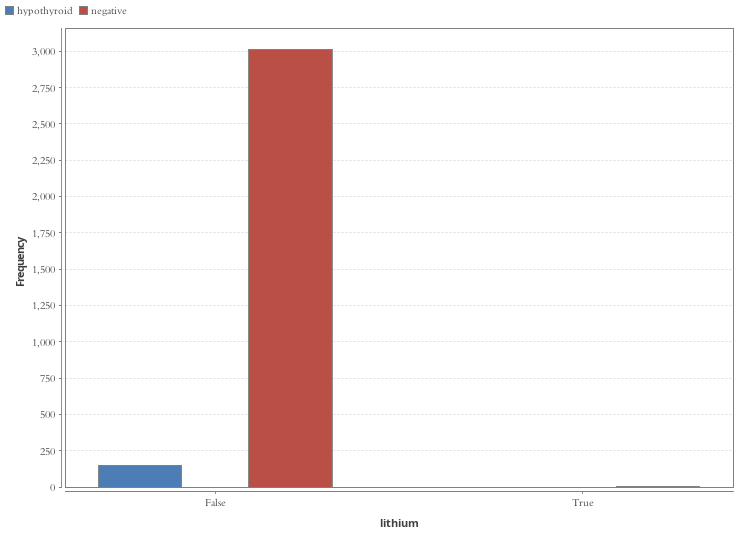
\includegraphics[width=0.45\textwidth]{analysis/histogram_lithium}
    \caption{Histograma del atributo \textit{lithium}.}
    \label{figure:histogram_lithium}
\end{figure}

\begin{figure}[H]
    \centering
    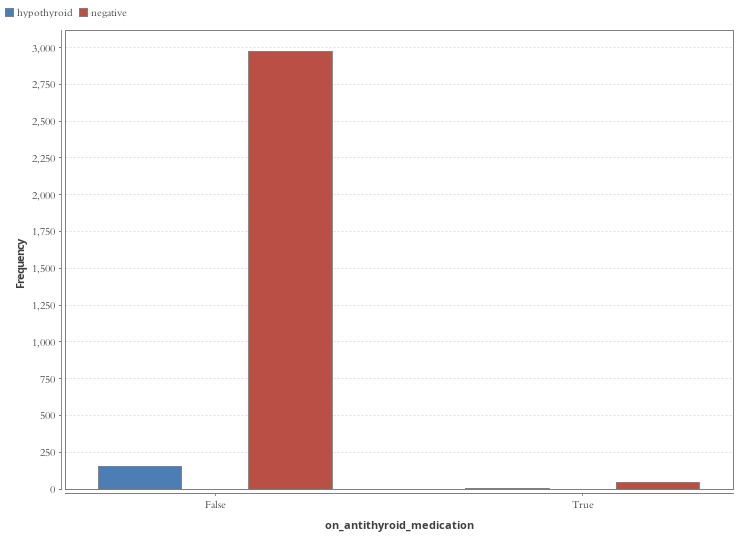
\includegraphics[width=0.45\textwidth]{analysis/histogram_on_antithyroid_medication}
    \caption{Histograma del atributo \textit{on\_antithyroid\_medication}.}
    \label{figure:on_antithyroid_medication}
\end{figure}

\begin{figure}[H]
    \centering
    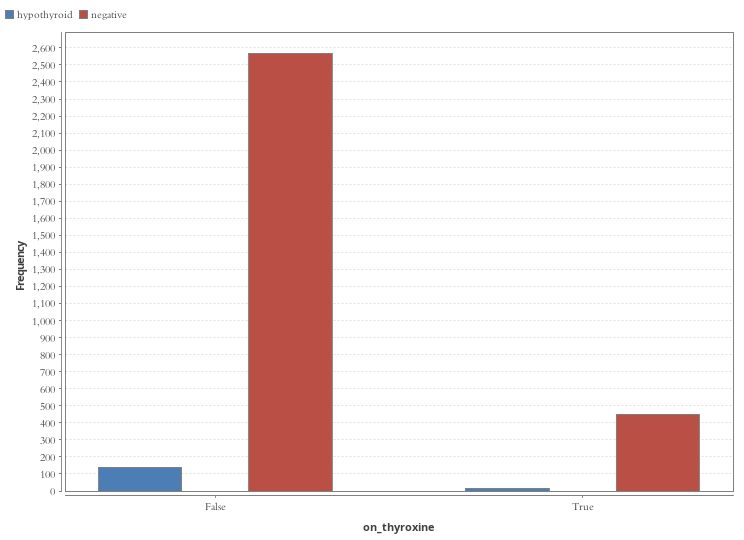
\includegraphics[width=0.45\textwidth]{analysis/histogram_on_thyroxine}
    \caption{Histograma del atributo \textit{on\_thyroxine}.}
    \label{figure:on_thyroxine}
\end{figure}

\begin{figure}[H]
    \centering
    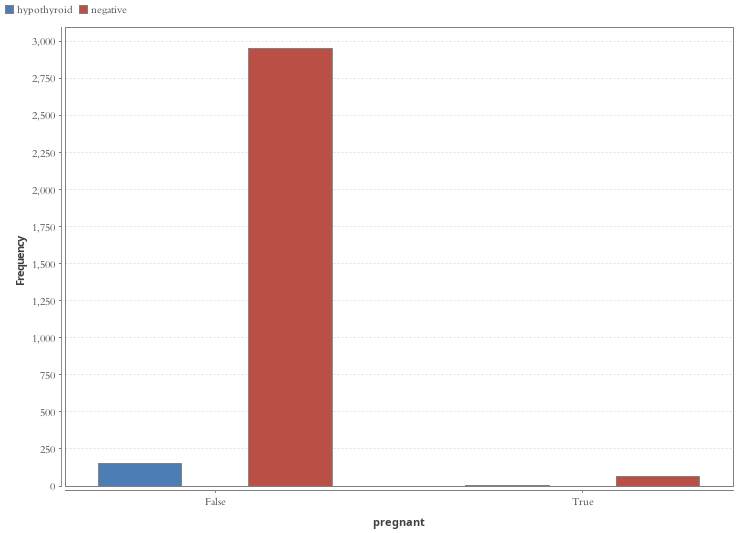
\includegraphics[width=0.45\textwidth]{analysis/histogram_pregnant}
    \caption{Histograma del atributo \textit{pregnant}.}
    \label{figure:pregnant}
\end{figure}

\begin{figure}[H]
    \centering
    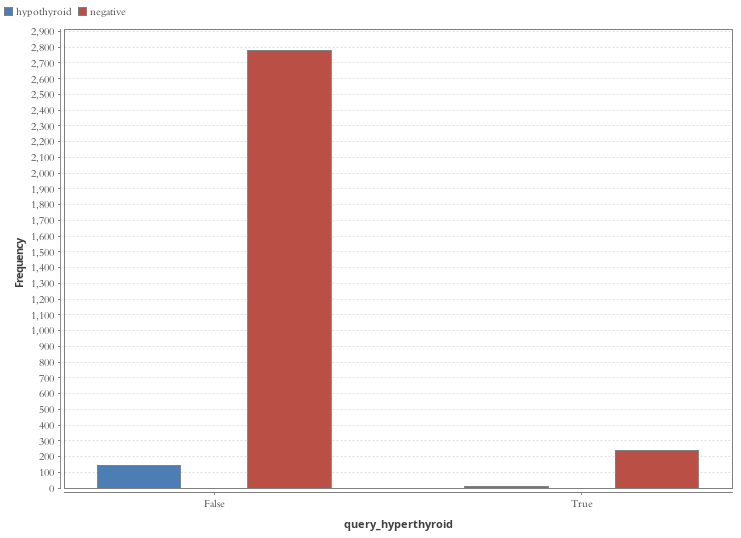
\includegraphics[width=0.45\textwidth]{analysis/histogram_query_hyperthyroid}
    \caption{Histograma del atributo \textit{query\_hyperthyroid}.}
    \label{figure:query_hyperthyroid}
\end{figure}

\begin{figure}[H]
    \centering
    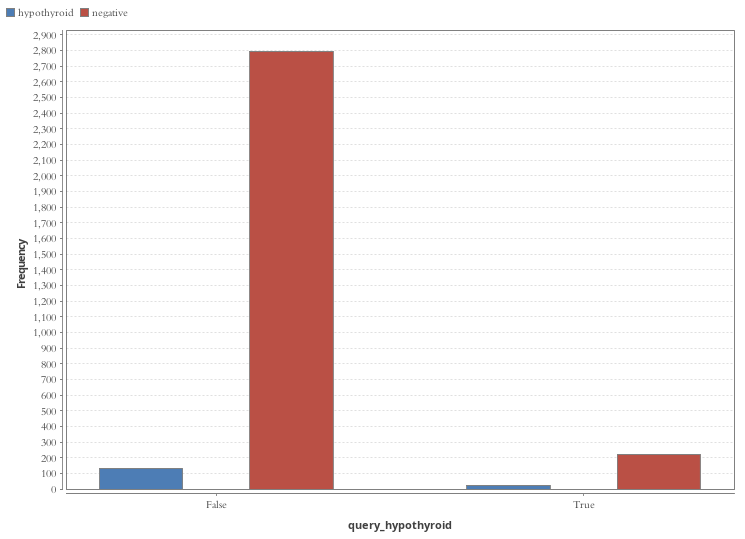
\includegraphics[width=0.45\textwidth]{analysis/histogram_query_hypothyroid}
    \caption{Histograma del atributo \textit{query\_hypothyroid}.}
    \label{figure:query_hypothyroid}
\end{figure}

\begin{figure}[H]
    \centering
    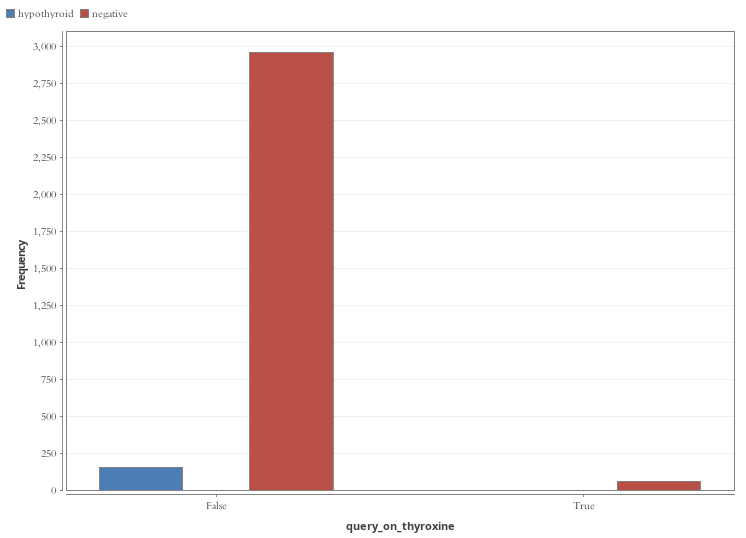
\includegraphics[width=0.45\textwidth]{analysis/histogram_query_on_thyroxine}
    \caption{Histograma del atributo \textit{query\_on\_thyroxine}.}
    \label{figure:query_on_thyroxine}
\end{figure}

\begin{figure}[H]
    \centering
    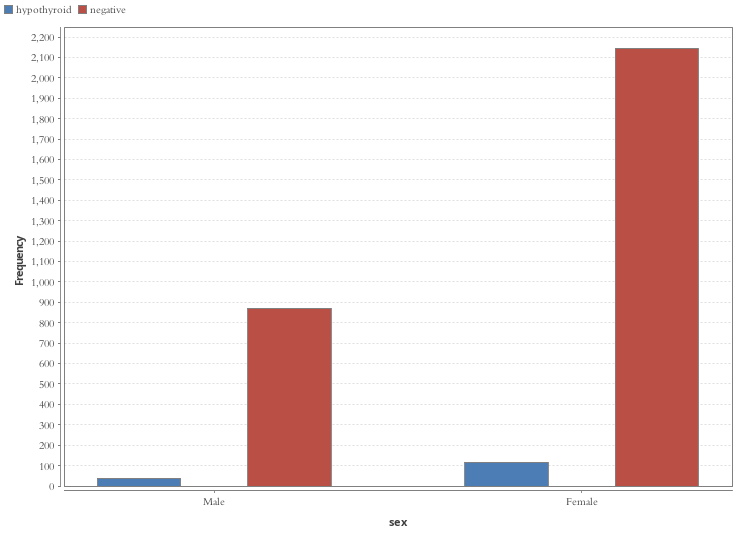
\includegraphics[width=0.45\textwidth]{analysis/histogram_sex}
    \caption{Histograma del atributo \textit{sex}.}
    \label{figure:sex}
\end{figure}

\begin{figure}[H]
    \centering
    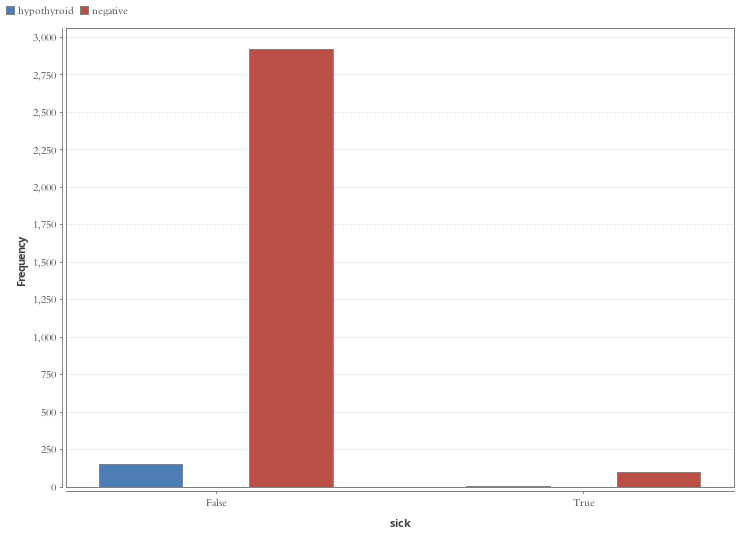
\includegraphics[width=0.45\textwidth]{analysis/histogram_sick}
    \caption{Histograma del atributo \textit{sick}.}
    \label{figure:sick}
\end{figure}

\begin{figure}[H]
    \centering
    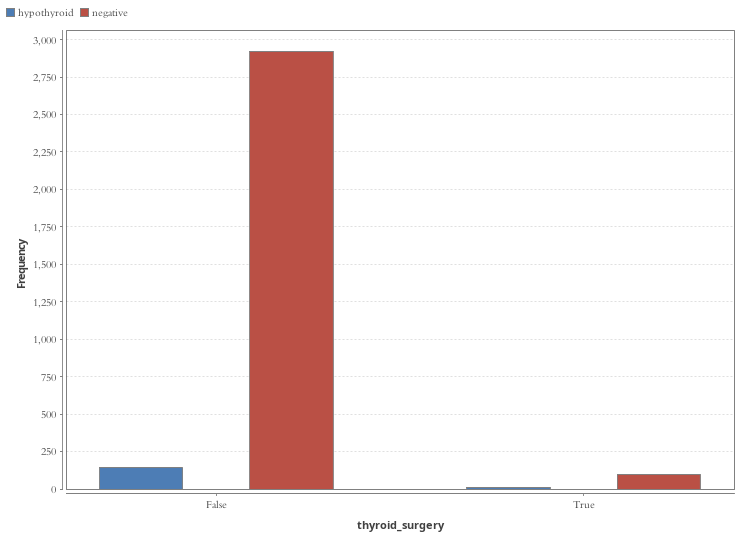
\includegraphics[width=0.45\textwidth]{analysis/histogram_thyroid_surgery}
    \caption{Histograma del atributo \textit{thyroid\_surgery}.}
    \label{figure:thyroid_surgery}
\end{figure}

\begin{figure}[H]
    \centering
    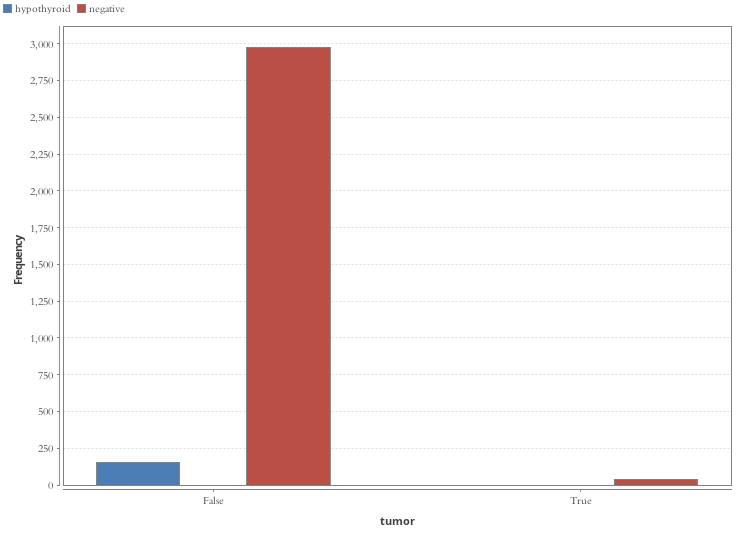
\includegraphics[width=0.45\textwidth]{analysis/histogram_tumor}
    \caption{Histograma del atributo \textit{tumor}.}
    \label{figure:tumor}
\end{figure}

\begin{figure}[H]
    \centering
    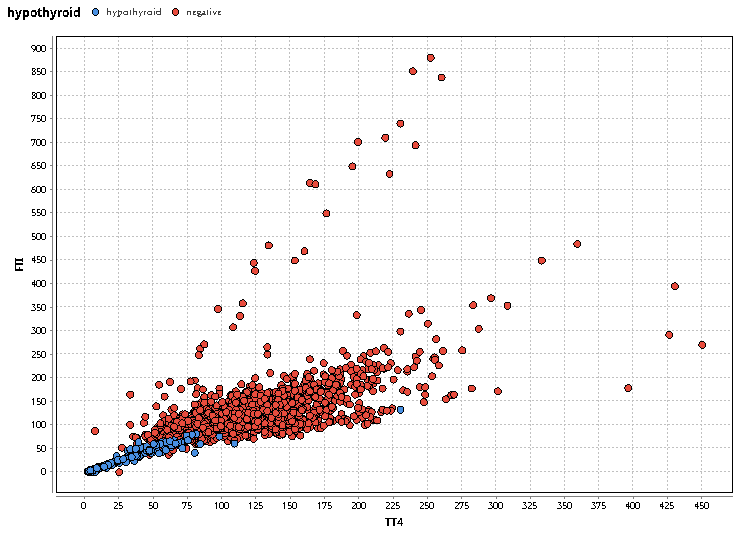
\includegraphics[width=0.45\textwidth]{analysis/scatter_TT4_FTI}
    \caption{Diagrama de dispersión de los atributos \textit{TT4, FTI}.}
    \label{figure:scatter_TT4_FTI}
\end{figure}

\begin{figure}[H]
    \centering
    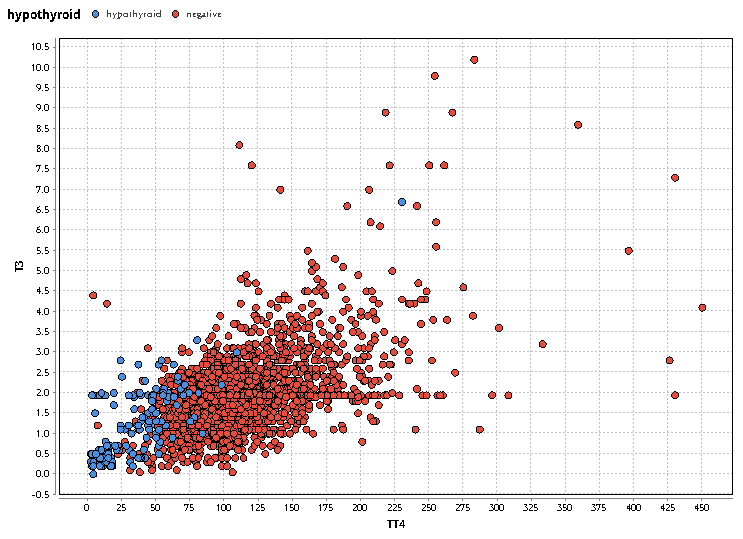
\includegraphics[width=0.45\textwidth]{analysis/scatter_TT4_T3}
    \caption{Diagrama de dispersión de los atributos \textit{TT4, T3}.}
    \label{figure:scatter_TT4_T3}
\end{figure}

\begin{figure}[H]
    \centering
    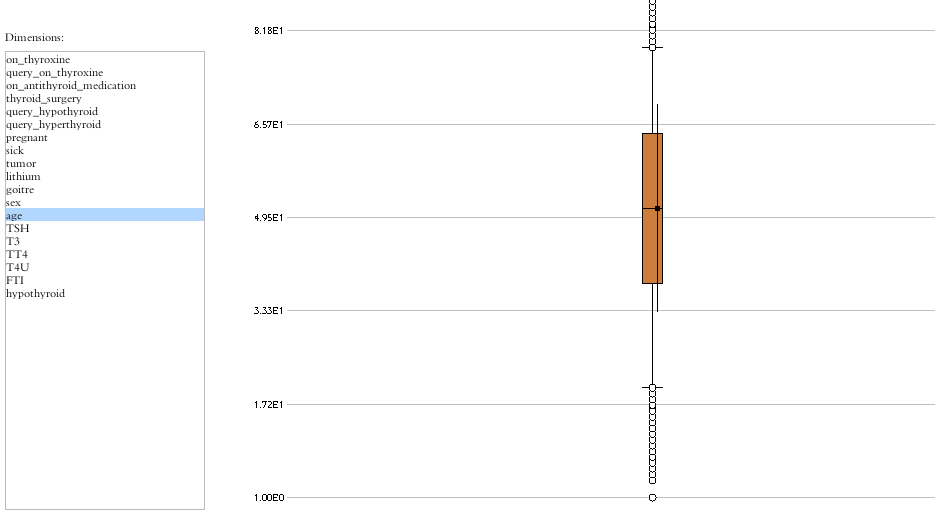
\includegraphics[width=0.45\textwidth]{analysis/box_plot_age}
    \caption{Diagrama de cajas del atributo \textit{age}.}
    \label{figure:box_plot_age}
\end{figure}

\begin{figure}[H]
    \centering
    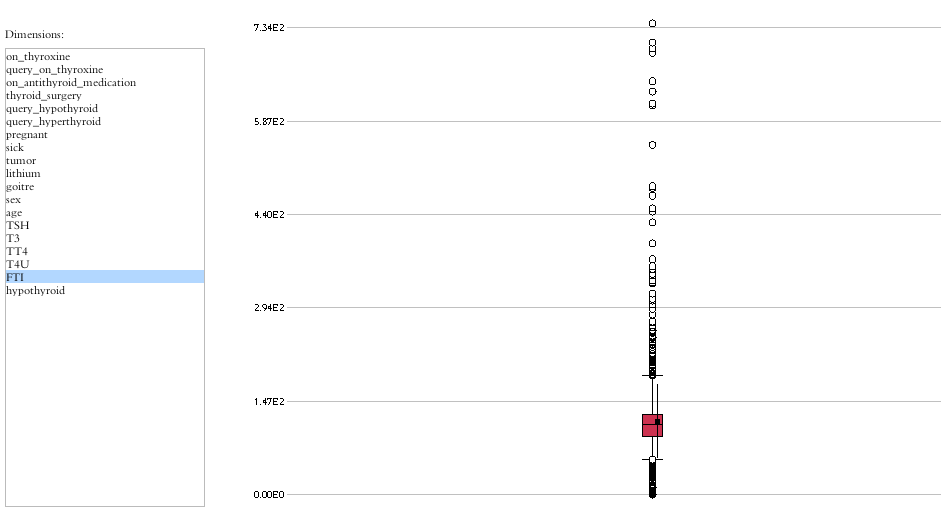
\includegraphics[width=0.45\textwidth]{analysis/box_plot_FTI}
    \caption{Diagrama de cajas del atributo \textit{FTI}.}
    \label{figure:box_plot_FTI}
\end{figure}

\begin{figure}[H]
    \centering
    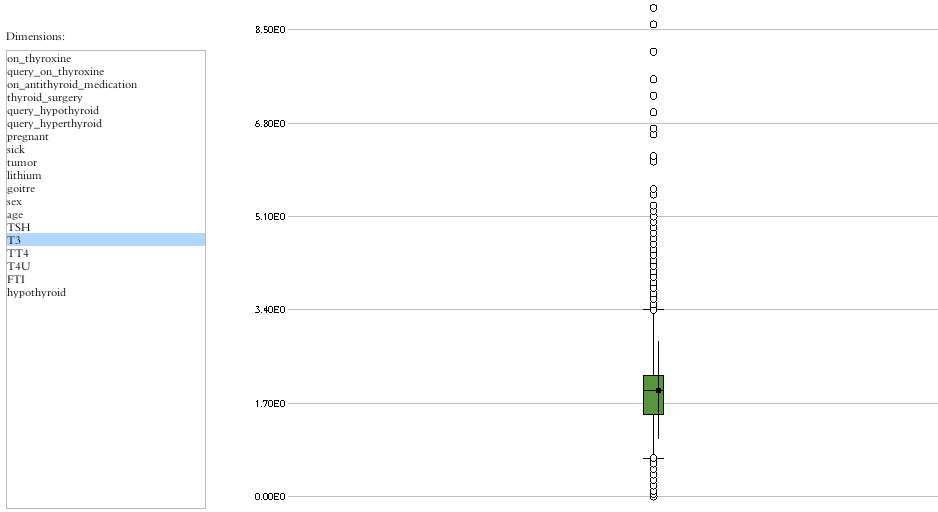
\includegraphics[width=0.45\textwidth]{analysis/box_plot_T3}
    \caption{Diagrama de cajas del atributo \textit{T3}.}
    \label{figure:box_plot_T3}
\end{figure}

\begin{figure}[H]
    \centering
    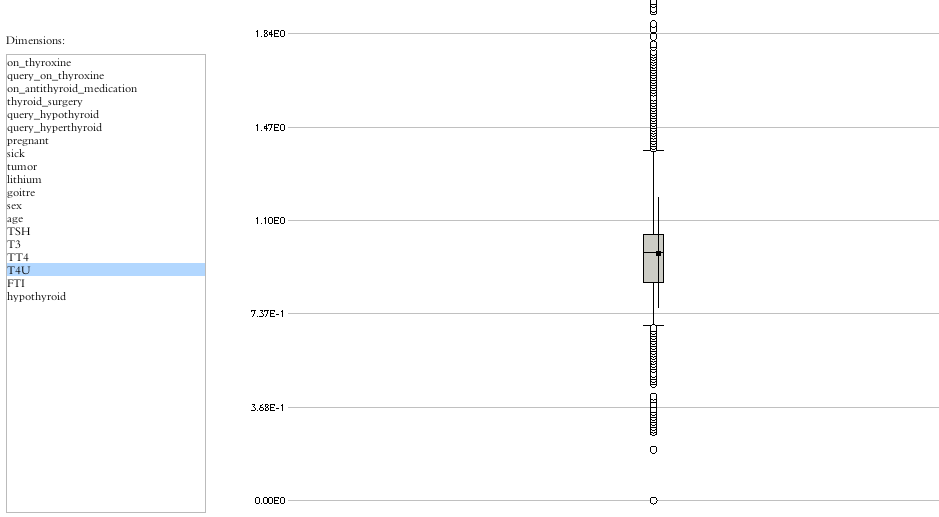
\includegraphics[width=0.45\textwidth]{analysis/box_plot_T4U}
    \caption{Diagrama de cajas del atributo \textit{T4U}.}
    \label{figure:box_plot_T4U}
\end{figure}

\begin{figure}[H]
    \centering
    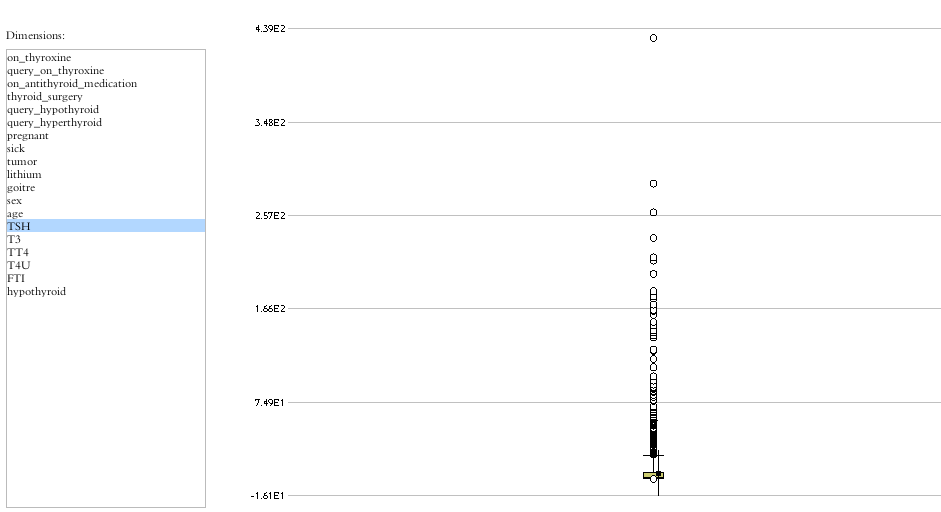
\includegraphics[width=0.45\textwidth]{analysis/box_plot_TSH}
    \caption{Diagrama de cajas del atributo \textit{TSH}.}
    \label{figure:box_plot_TSH}
\end{figure}

\onecolumngrid

\clearpage

\subsection{Modelos y Performance}

\subsubsection{Modelos} \label{apendix:models:models} 

\begin{table}[ht]
    \begin{tabular}{|l|l|l|}
        \hline
        Atributo & cluster\_0 & cluster\_1 \\
        \hline
        
        sex = M & 0.10256410256410256 & 0.2893725992317542 \\
        sex = F & 0.8974358974358975 & 0.7106274007682458 \\
        on\_thyroxine = f & 0.9487179487179487 & 0.8530729833546735 \\
        on\_thyroxine = t & 0.05128205128205128 & 0.1469270166453265 \\
        query\_on\_thyroxine = f & 1.0 & 0.9823943661971831 \\
        query\_on\_thyroxine = t & 0.0 & 0.017605633802816902 \\
        on\_antithyroid\_medication = f & 1.0 & 0.9865556978233034 \\
        on\_antithyroid\_medication = t & 0.0 & 0.013444302176696543 \\
        thyroid\_surgery = f & 1.0 & 0.9667093469910372 \\
        thyroid\_surgery = t & 0.0 & 0.03329065300896287 \\
        query\_hypothyroid = f & 0.9487179487179487 & 0.9234955185659411 \\
        query\_hypothyroid = t & 0.05128205128205128 & 0.0765044814340589 \\
        query\_hyperthyroid = f & 0.6923076923076923 & 0.926056338028169 \\
        query\_hyperthyroid = t & 0.3076923076923077 & 0.07394366197183098 \\
        pregnant = f & 0.9743589743589743 & 0.9801536491677336 \\
        pregnant = t & 0.02564102564102564 & 0.019846350832266324 \\
        sick = f & 1.0 & 0.9683098591549296 \\
        sick = t & 0.0 & 0.03169014084507042 \\
        tumor = f & 1.0 & 0.9871959026888605 \\
        tumor = t & 0.0 & 0.012804097311139564 \\
        lithium = f & 1.0 & 0.9993597951344431 \\
        lithium = t & 0.0 & 6.402048655569782E-4 \\
        goitre = f & 1.0 & 0.9683098591549296 \\
        goitre = t & 0.0 & 0.03169014084507042 \\
        age & 51.51282051282051 & 51.127720870678615 \\
        TSH & 4.964323581180723 & 5.935150321052643 \\
        T3 & 3.487115072933549 & 1.920431471620351 \\
        TT4 & 249.64102564102564 & 107.09236555697822 \\
        T4U & 0.616923076923077 & 0.9827091372498201 \\
        FTI & 472.56410256410254 & 110.93890826408756 \\
        \hline
    \end{tabular}
    \caption{Agrupamiento generado por el algoritmo \textit{k-means}}
    \label{table:k_means_model}
\end{table}

\subsubsection{Performance} \label{apendix:models:performance} 

\begin{figure}[h]
    \centering
    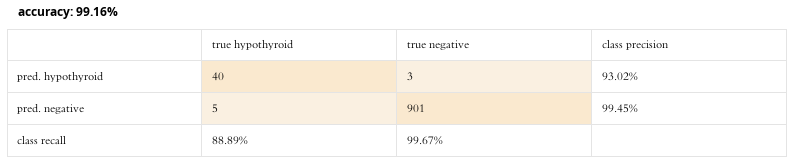
\includegraphics[width=0.75\textwidth]{models/w_j48_performance}
    \caption{Performance del modelo de Árbol generado utilizando el algoritmo C4.5 sobre un conjunto de testeo correspondiente al 30\% del conjunto total de datos.}
    \label{figure:w_j48_performance}
\end{figure}

\begin{figure}[h]
    \centering
    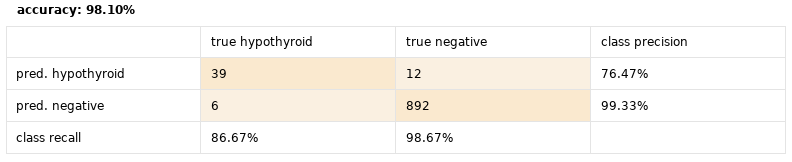
\includegraphics[width=0.75\textwidth]{models/w_oneR_performance}
    \caption{Performance del modelo de reglas generado utilizando el algoritmo OneR sobre un conjunto de testeo correspondiente al 30\% del conjunto total de datos.}
    \label{figure:w_oneR_performance}
\end{figure}

\begin{figure}[h]
    \centering
    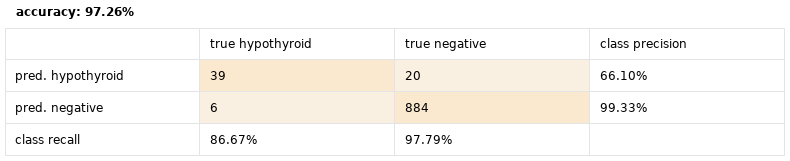
\includegraphics[width=0.75\textwidth]{models/prism_performance}
    \caption{Performance del modelo de reglas generado utilizando el algoritmo PRISM sobre un conjunto de testeo correspondiente al 30\% del conjunto total de datos.}
    \label{figure:prism_performance}
\end{figure}

\begin{figure}[h]
    \centering
    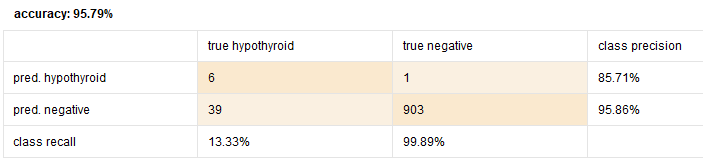
\includegraphics[width=0.75\textwidth]{models/perceptron_performance}
    \caption{Performance del modelo de redes neuronales generado utilizando la arquitectura perceptron sobre un conjunto de testeo correspondiente al 30\% del conjunto total de datos.}
    \label{figure:perceptron_performance}
\end{figure}

\begin{figure}[h]
    \centering
    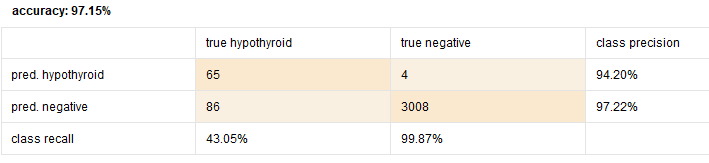
\includegraphics[width=0.75\textwidth]{models/perceptron_train_test_performance}
    \caption{Performance del modelo de redes neuronales generado utilizando la arquitectura perceptron sobre un conjunto de testeo correspondiente conjunto total de datos de entrenamiento.}
    \label{figure:perceptron_train_test_performance}
\end{figure}

\begin{figure}[h]
    \centering
    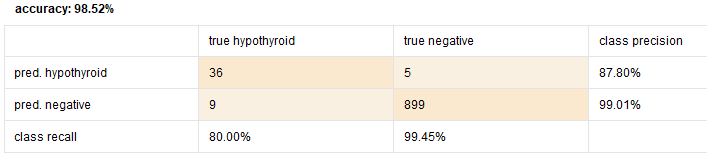
\includegraphics[width=0.75\textwidth]{models/multiperceptron_performance}
    \caption{Performance del modelo de redes neuronales generado utilizando la arquitectura multiperceptron sobre un conjunto de testeo correspondiente al 30\% del conjunto total de datos.}
    \label{figure:multiperceptron_performance}
\end{figure}

\begin{figure}[h]
    \centering
    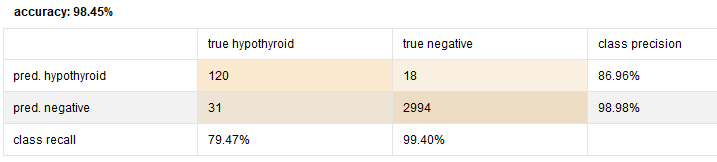
\includegraphics[width=0.75\textwidth]{models/multiperceptron_train_test_performance}
    \caption{Performance del modelo de redes neuronales generado utilizando la arquitectura multiperceptron sobre un conjunto de testeo correspondiente al conjunto total de datos de entrenamiento.}
    \label{figure:multiperceptron_train_test_performance}
\end{figure}

\end{document}
